\documentclass{ximera}

%\addPrintStyle{..}

\begin{document}
	\author{Bart Lambregs}
	\xmtitle{Oefeningen kinematica}{}
    \xmsource\xmuitleg




\begin{exercise}
Kan de snelheid van een voorwerp gelijk zijn aan nul, terwijl de versnelling verschillend is van nul? Motiveer je antwoord.
\end{exercise}


\begin{exercise}
Kan een voorwerp dat een positieve versnelling heeft een negatieve snelheid hebben? Kan het omgekeerde ook? Licht je antwoord toe.

\begin{oplossing}
    Ja, dat kan. Neem bijvoorbeeld een voorwerp dat je verticaal omhoog gooit. Als je de referentieas waarmee je de beweging wil beschrijven verticaal naar benden kiest, zal de versnelling van de beweging positief zijn en de snelheid negatief. De snelheid is negatief omdat je tegengesteld aan de as beweegt en de versnelling is positief omdat de snelheid minder negatief wordt.

    Het omgekeerde kan ook, draai gewoon de referentieas om.
\end{oplossing}
\end{exercise}

\begin{exercise}
	Een puntmassa beweegt volgens de plaatsfunctie
	\[
	x(t)=t^3-3t^2-10t
	\]
	Bereken haar snelheidscomponent telkens als ze het vertrekpunt passeert. Hoe groot is dan de versnellingscomponent?
	\begin{oplossing}
		$x=t(t-5)(t+2)$
	\end{oplossing}
\end{exercise}


\begin{exercise}

Een veerman tracht een stromende rivier loodrecht over te roeien. 
Hij slaagt erin ten opzicht van het water een snelheid van $2,00\rm\,m/s$ te ontwikkelen -- de stroomsnelheid is \SI{1,25}{m/s}. 
De rivier is \SI{150}{\meter} breed. 

\begin{question}
 Onder welke hoek ten opzichte van de loodlijn op de oever moet hij steeds blijven roeien?
\begin{oplossing}
Er is gegeven dat

\begin{itemize}
	\item $v_1=\SI{2}{\meter\per\second}$
	\item$v_2=\SI{1,25}{\meter\per\second}$
	\item $d=\SI{150}{\meter}$
\end{itemize}

We berekenen de hoek $\alpha$. 


De component, tegengesteld aan de stroomrichting, van de snelheid waarmee de veerman roeit ten opzichte van het water, moet even groot zijn als de stroomsnelheid zodat hij in de richting van de rivier resulterend
geen snelheid zal hebben. 

% \begin{figure}[h]
% \centering
% 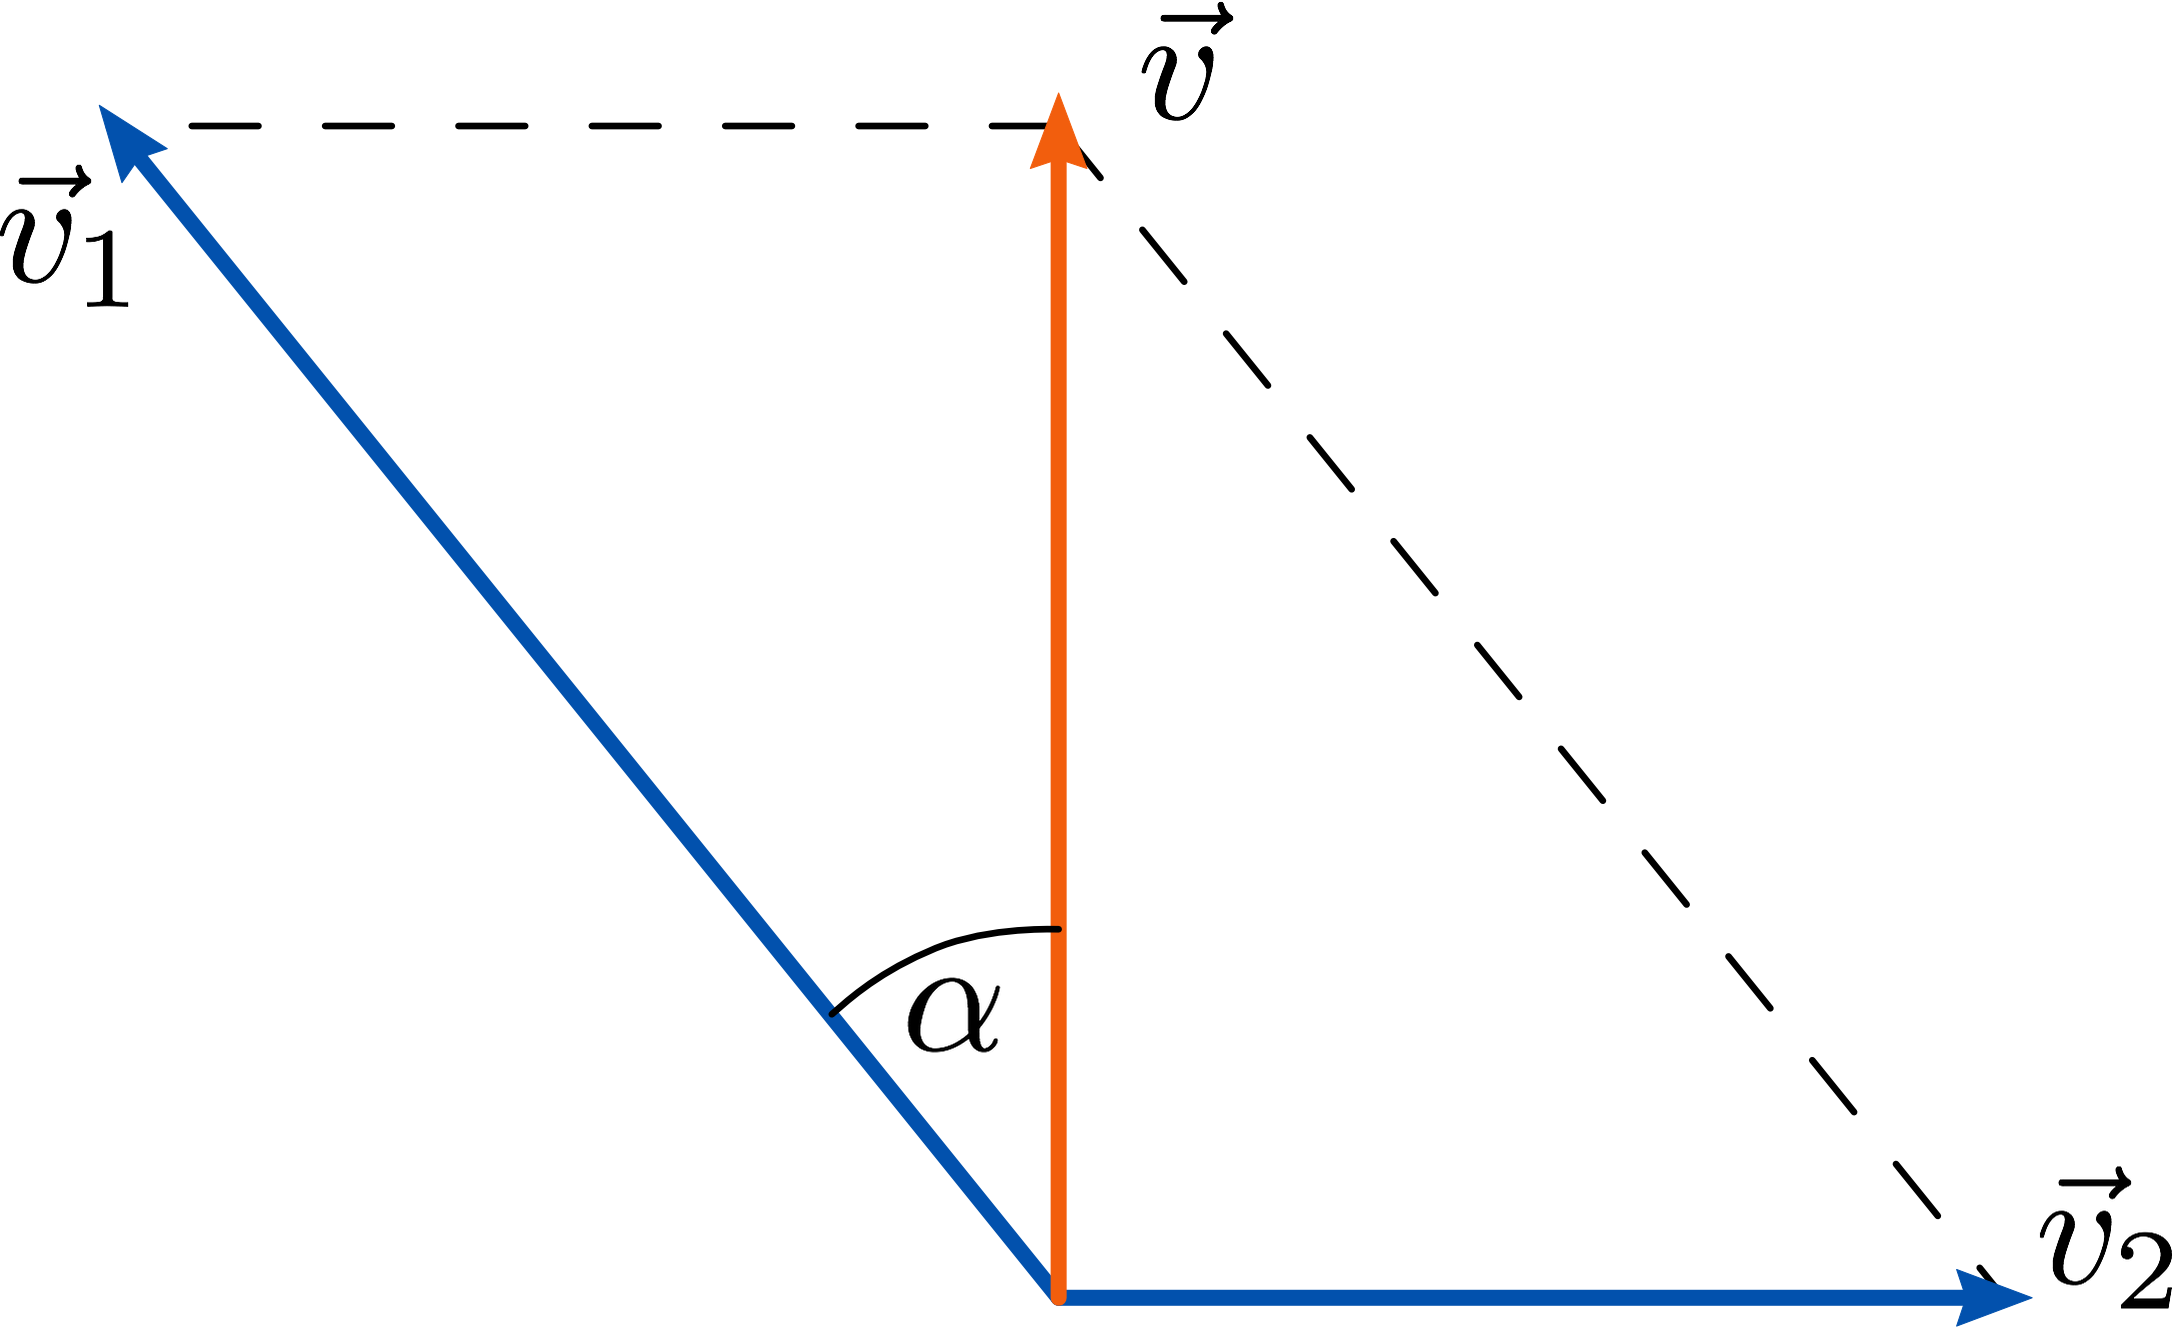
\includegraphics[width=0.45\textwidth]{dyn/exercises/vectoren_veerman}
% \end{figure}

De hoek vinden we dan als volgt (zie figuur):

\begin{align*}
\sin{\alpha} &= \frac{v_2}{v_1}\\
&\Downarrow\\
\alpha&=\bgsin\left(\frac{v_2}{v_1}\right)\\
&=38,7^\circ
\end{align*}

\end{oplossing}

\end{question}
\begin{question}
Hoeveel tijd heeft de veerman nodig om de overzijde te bereiken? 

\begin{oplossing}
De tijd nodig om de overzijde te bereiken vinden we door zijn snelheid loodrecht op de oever -- zijn resulterende snelheid $v$ -- te bekijken:
	\begin{align*}
		%v&=&v_1\cos{\alpha}\qquad\left(=v_1\cos\left(\bgsin\left(\frac{v_2}{v_1}\right)\right)=v_1\sqrt{1-\left(\frac{v_2}{v_1}\right)^2}=\sqrt{v_1^2-v_2^2}\right)\\
		%&\Downarrow&\\
		t=\frac{d}{v}=\frac{d}{\sqrt{v_1^2-v_2^2}}=96,1{\rm\,s}
	\end{align*}

\end{oplossing}
\end{question}
\end{exercise}

\begin{exercise}
De coördinaten van een deeltje zijn als functie van de tijd wordt gegeven door
\[
\left\{
\begin{aligned}
	x&=t^2 \\
	y&=t^2
\end{aligned}
\right.
\]

\begin{multipleChoice}
\choice{Dan is de versnelling steeds evenwijdig aan de $x$-as.}
\choice{Dan is de versnelling steeds evenwijdig aan de $y$-as.}
\choice[correct]{Dan maakt de versnelling steeds een hoek van $45^\circ$ met de $x$-as.}
\choice{Dan wordt het deeltje niet versneld}
\end{multipleChoice}
\end{exercise}

\begin{exercise}
	De positie van een deeltje als functie van de tijd wordt beschreven door
	\[
	\vec{r}=bt\vec{e}_x+(c-dt^2)\vec{e}_y
	\]
	met $b=2,00\rm\,m/s$, $c=5,00\rm\,m$ en $d=1,00\rm\,m/s^2$.
	
	\begin{question}
	Druk $y$ uit in functie van $x$. Hoe ziet de baan eruit?
	
	\begin{oplossing}
	We moeten dus de baanvergelijking geven. 
	Dit doen we door de tijd uit te drukken i.f.v. de positie $x$ en dit te substitueren in de coördinaatvergelijking $y(t)$.
	\begin{align*}
	x&=bt \quad \Leftrightarrow \quad t=\frac{x}{b}\\
	&\Downarrow\\
	y&=c-dt^2=c-\frac{d}{b^2}x^2
	\end{align*}
	Dit is een bergparabool met top $(0,c)=(0,5,00\rm\,m)$.
	\end{oplossing}
	\end{question}
	
	\begin{question}
	Bepaal de snelheidsvector.
	
	\begin{oplossing}
	De componenten van de snelheid zijn:
	\begin{align*}
	v_x&=\frac{dx}{dt}=b\\
	v_y&=\frac{dy}{dt}=-2dt
	\end{align*}
	zodat de snelheid(svector) wordt gegeven door
	\begin{align*}
	\vec{v}&=v_x\vec{e}_x+v_y\vec{e}_y\\
	&=b\vec{e}_x-2dt\vec{e}_y
	\end{align*}
	\end{oplossing}
	\end{question}
	
	\begin{question}
	Op welk tijdstip ($t>0$) staat de snelheid loodrecht op de plaatsvector?
	
	\begin{oplossing}
	De rechte die de richting van de snelheid weergeeft, staat loodrecht op de rechte die de richting van de positievector weergeeft wanneer het product van de richtingsco\"effici\"enten gelijk is aan $-1$:
	\begin{align*}
	rc_{r}\cdot rc_{v}&=-1\\
	&\Updownarrow\\
	\frac{y}{x}\cdot\frac{v_y}{v_x}&=-1\\
	&\Downarrow\\
	\frac{c-dt^2}{bt}\cdot\frac{-2dt}{b}&=-1\\
	&\Downarrow \quad (t>0)\\
	t&=\sqrt{\frac{2cd-b^2}{2d^2}}\\
	&=1,73\rm\,s
	\end{align*}
	\end{oplossing}
	\end{question}
	
	\end{exercise}
	


\begin{exercise}
	Een voorwerp maakt een beweging met volgende plaatscoördinaten:
	\[
	x=8t^{3},\qquad y=t^{6}-2,
	\]
	met \(x,y\) in \si{\meter} en \(t\) in \si{\second}.
	
	\begin{question}
	Bepaal de verplaatsing tussen \(t=\SI{0}{\second}\) en \(t=\SI{1}{\second}\).
	\end{question}
	
	\begin{question}
	Bepaal de snelheidsvector en de versnellingsvector op tijdstip \(t=\SI{1}{\second}\).
	\end{question}
	
	\begin{question}
	Is er op \(t=\SI{1}{\second}\) een tangentiële versnelling, een normale versnelling, of beide? Licht kort toe welke componenten aanwezig zijn.
	\end{question}
	
	\begin{question}
	Bepaal de baanvergelijking (weg van \(t\)) van het projectiel: schrijf \(y\) uit in functie van \(x\).
	\end{question}
	
	\end{exercise}
		


\end{document}
